% !TeX root = ../main.tex
% Add the above to each chapter to make compiling the PDF easier in some editors.

\chapter{Literature Review}\label{chapter:literaturereview}
This chapter provides a comprehensive review of the literature relevant to teleoperation interfaces for autonomous vehicles, focusing on environmental data visualization and perception modification. The review covers various topics, from the fundamentals of autonomous vehicle technology to specific teleoperation concepts and visualization approaches.
\section{Overview of Autonomous Vehicle Technology}

The Society of Automotive Engineers (SAE) International has defined six levels of
driving automation, as shown in figure 2.1 in their J3016 standard, which has become
the industry’s most widely accepted classification system. These levels range from 0
(no automation) to 5 (full automation), providing a clear framework for understanding
the capabilities of autonomous vehicles \cite{sae2021}

\begin{figure}[h]
    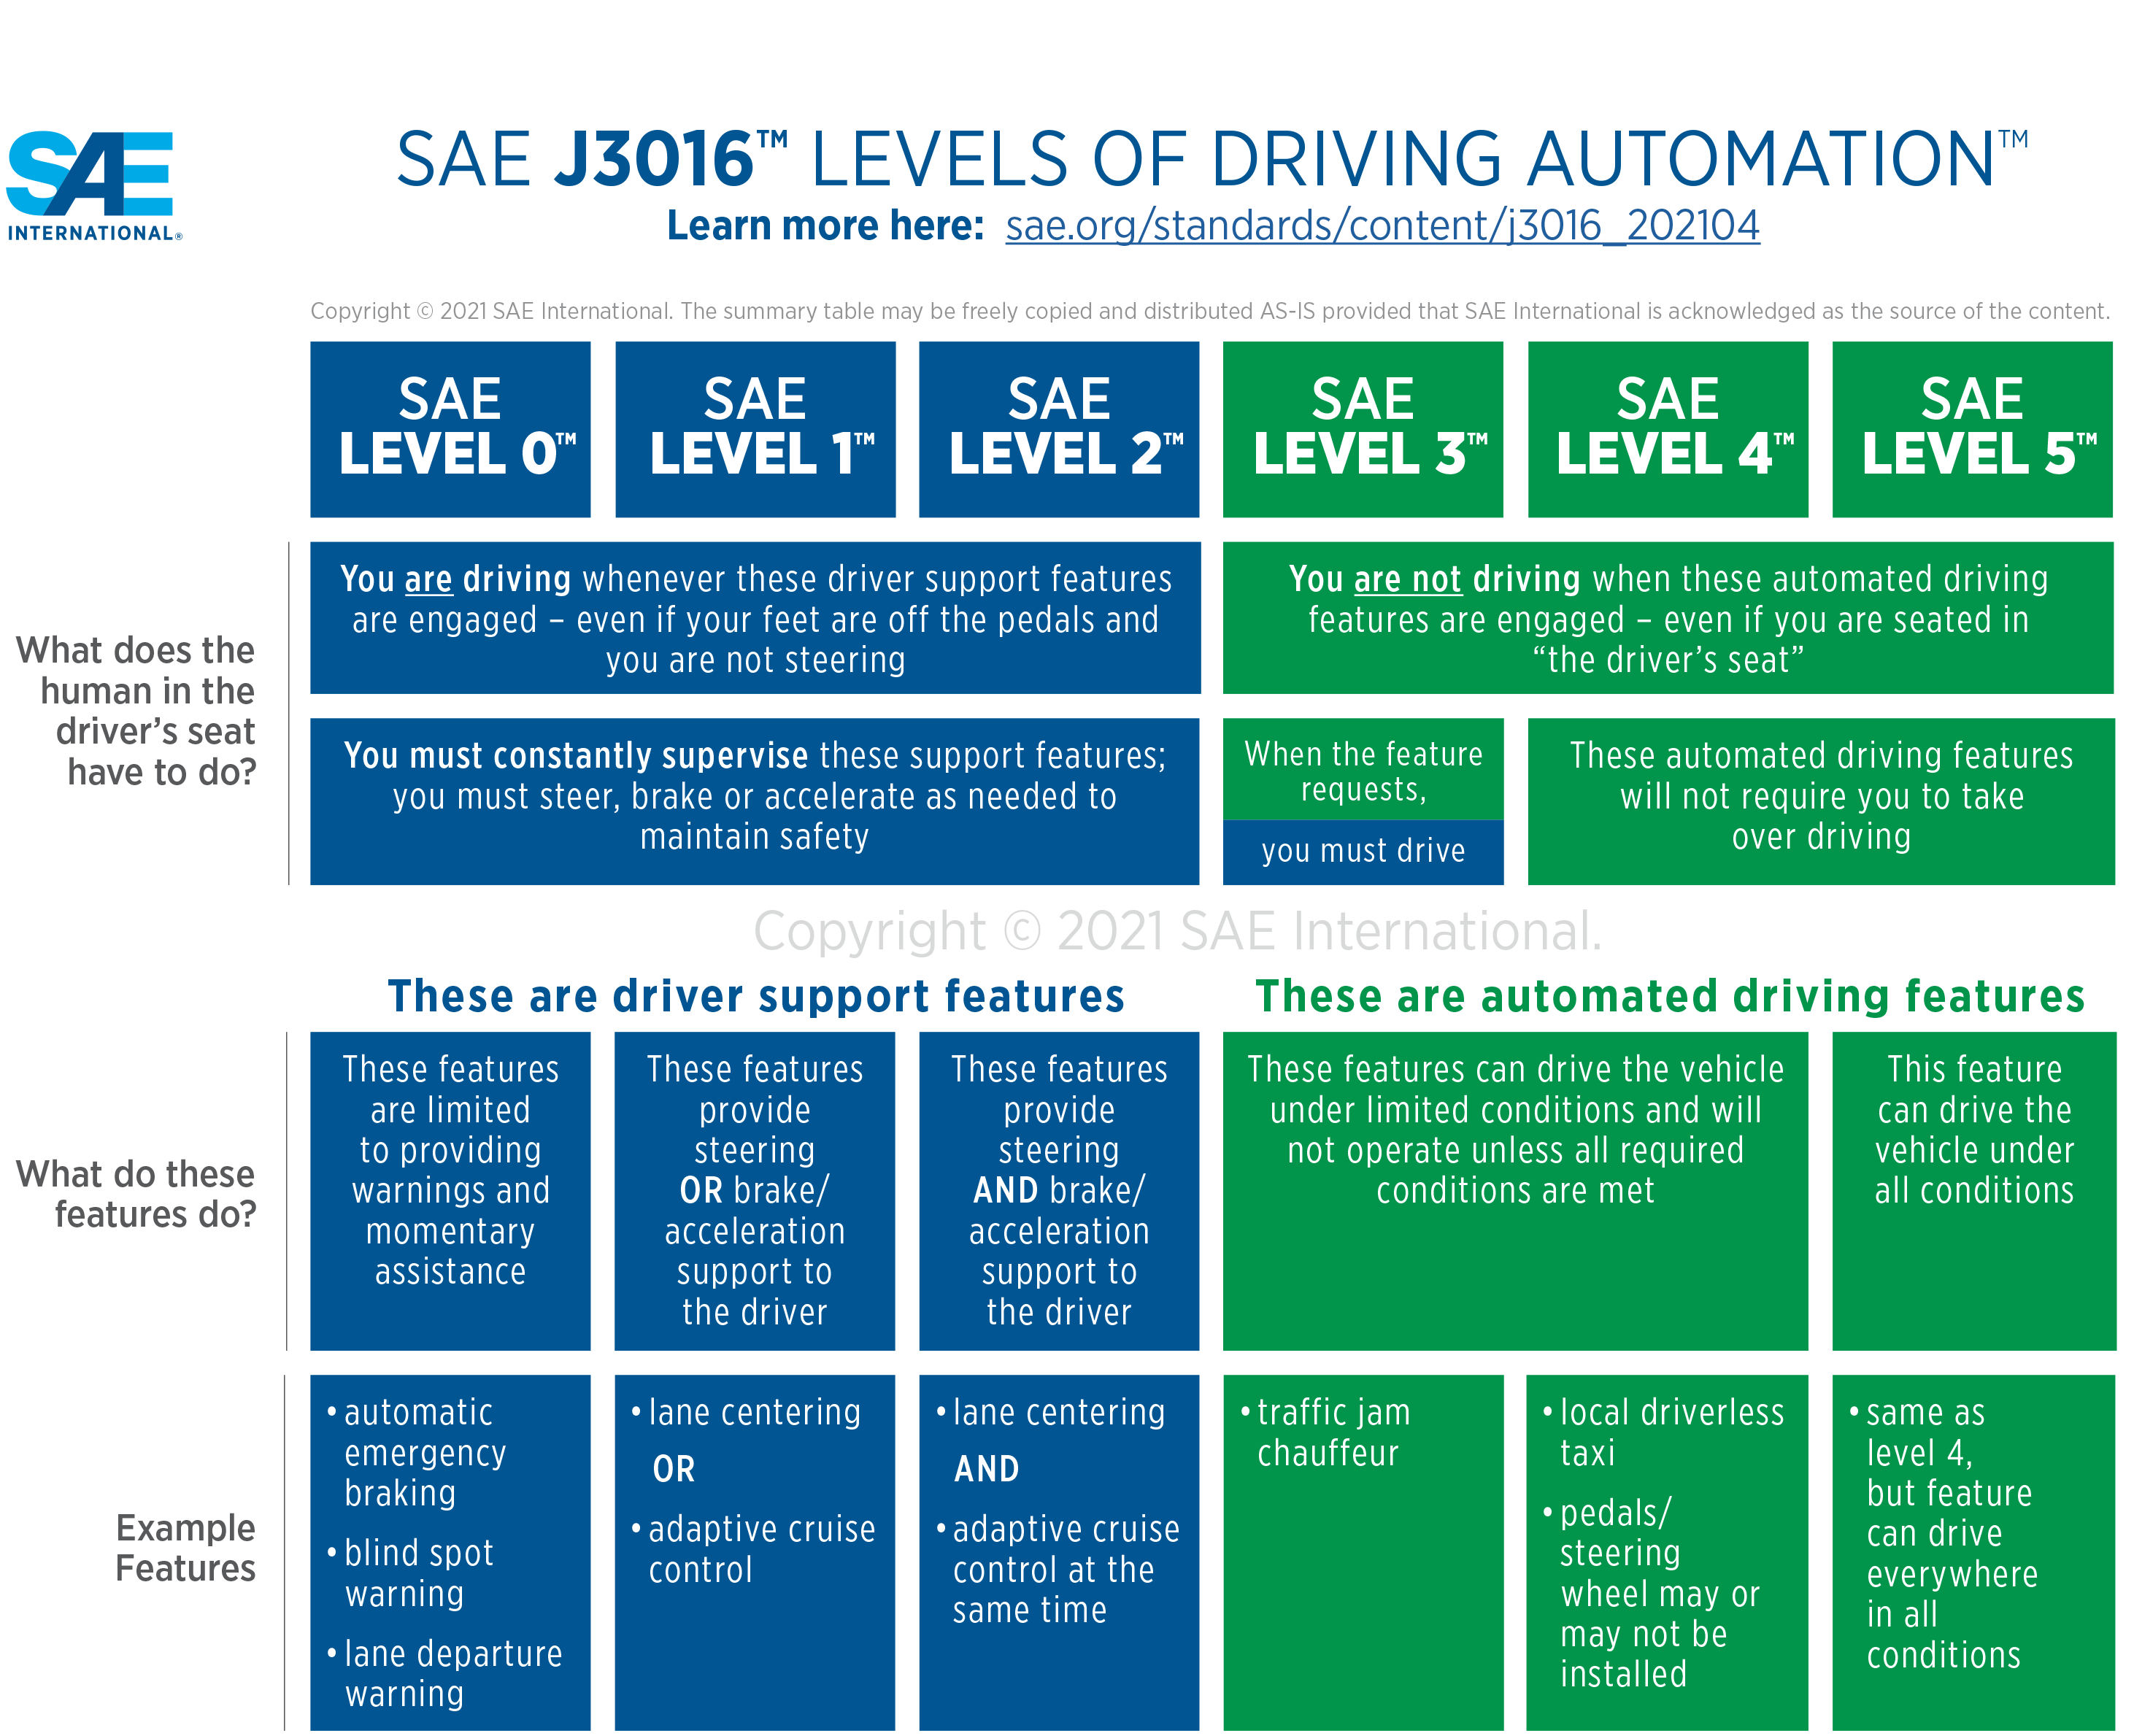
\includegraphics[scale=0.4]{figures/SAE.png}
    \centering
    \caption{SAE Levels of Automation \cite{sae2021}}
    \label{fig:SAE}
\end{figure}

As of 2024, most advanced consumer vehicles operate at Level 2, with some manufacturers pushing towards Level 3 capabilities. For example, BMW has recently become the first carmaker to receive approval for combining both Level 2 and Level 3 autonomous driving systems in a single vehicle. The new BMW 7 Series now offers the BMW Highway Assistant (Level 2) and the BMW Personal Pilot L3 (Level 3), marking a significant step in automated driving technology \cite{bmw2024}.

At the forefront of autonomous vehicle technology, companies like Waymo
are making significant strides towards Level 4 autonomy. Waymo has achieved
Level 4 autonomy in pilot areas, offering fully autonomous rides without safety
 drivers in cities like San Francisco, Phoenix, and Austin \cite{evmagazine2024}.

 Achieving higher SAE levels of autonomy requires a sophisticated autonomous driving stack,
 which is composed of several vital modules that work together to perceive the environment,
 make decisions, and control the vehicle. The stack typically follows a modular software
 architecture that is shown in Figure \ref{fig:AVStack} integrates hardware and software components to enable safe and
 efficient vehicle operation

\begin{figure}[h]
    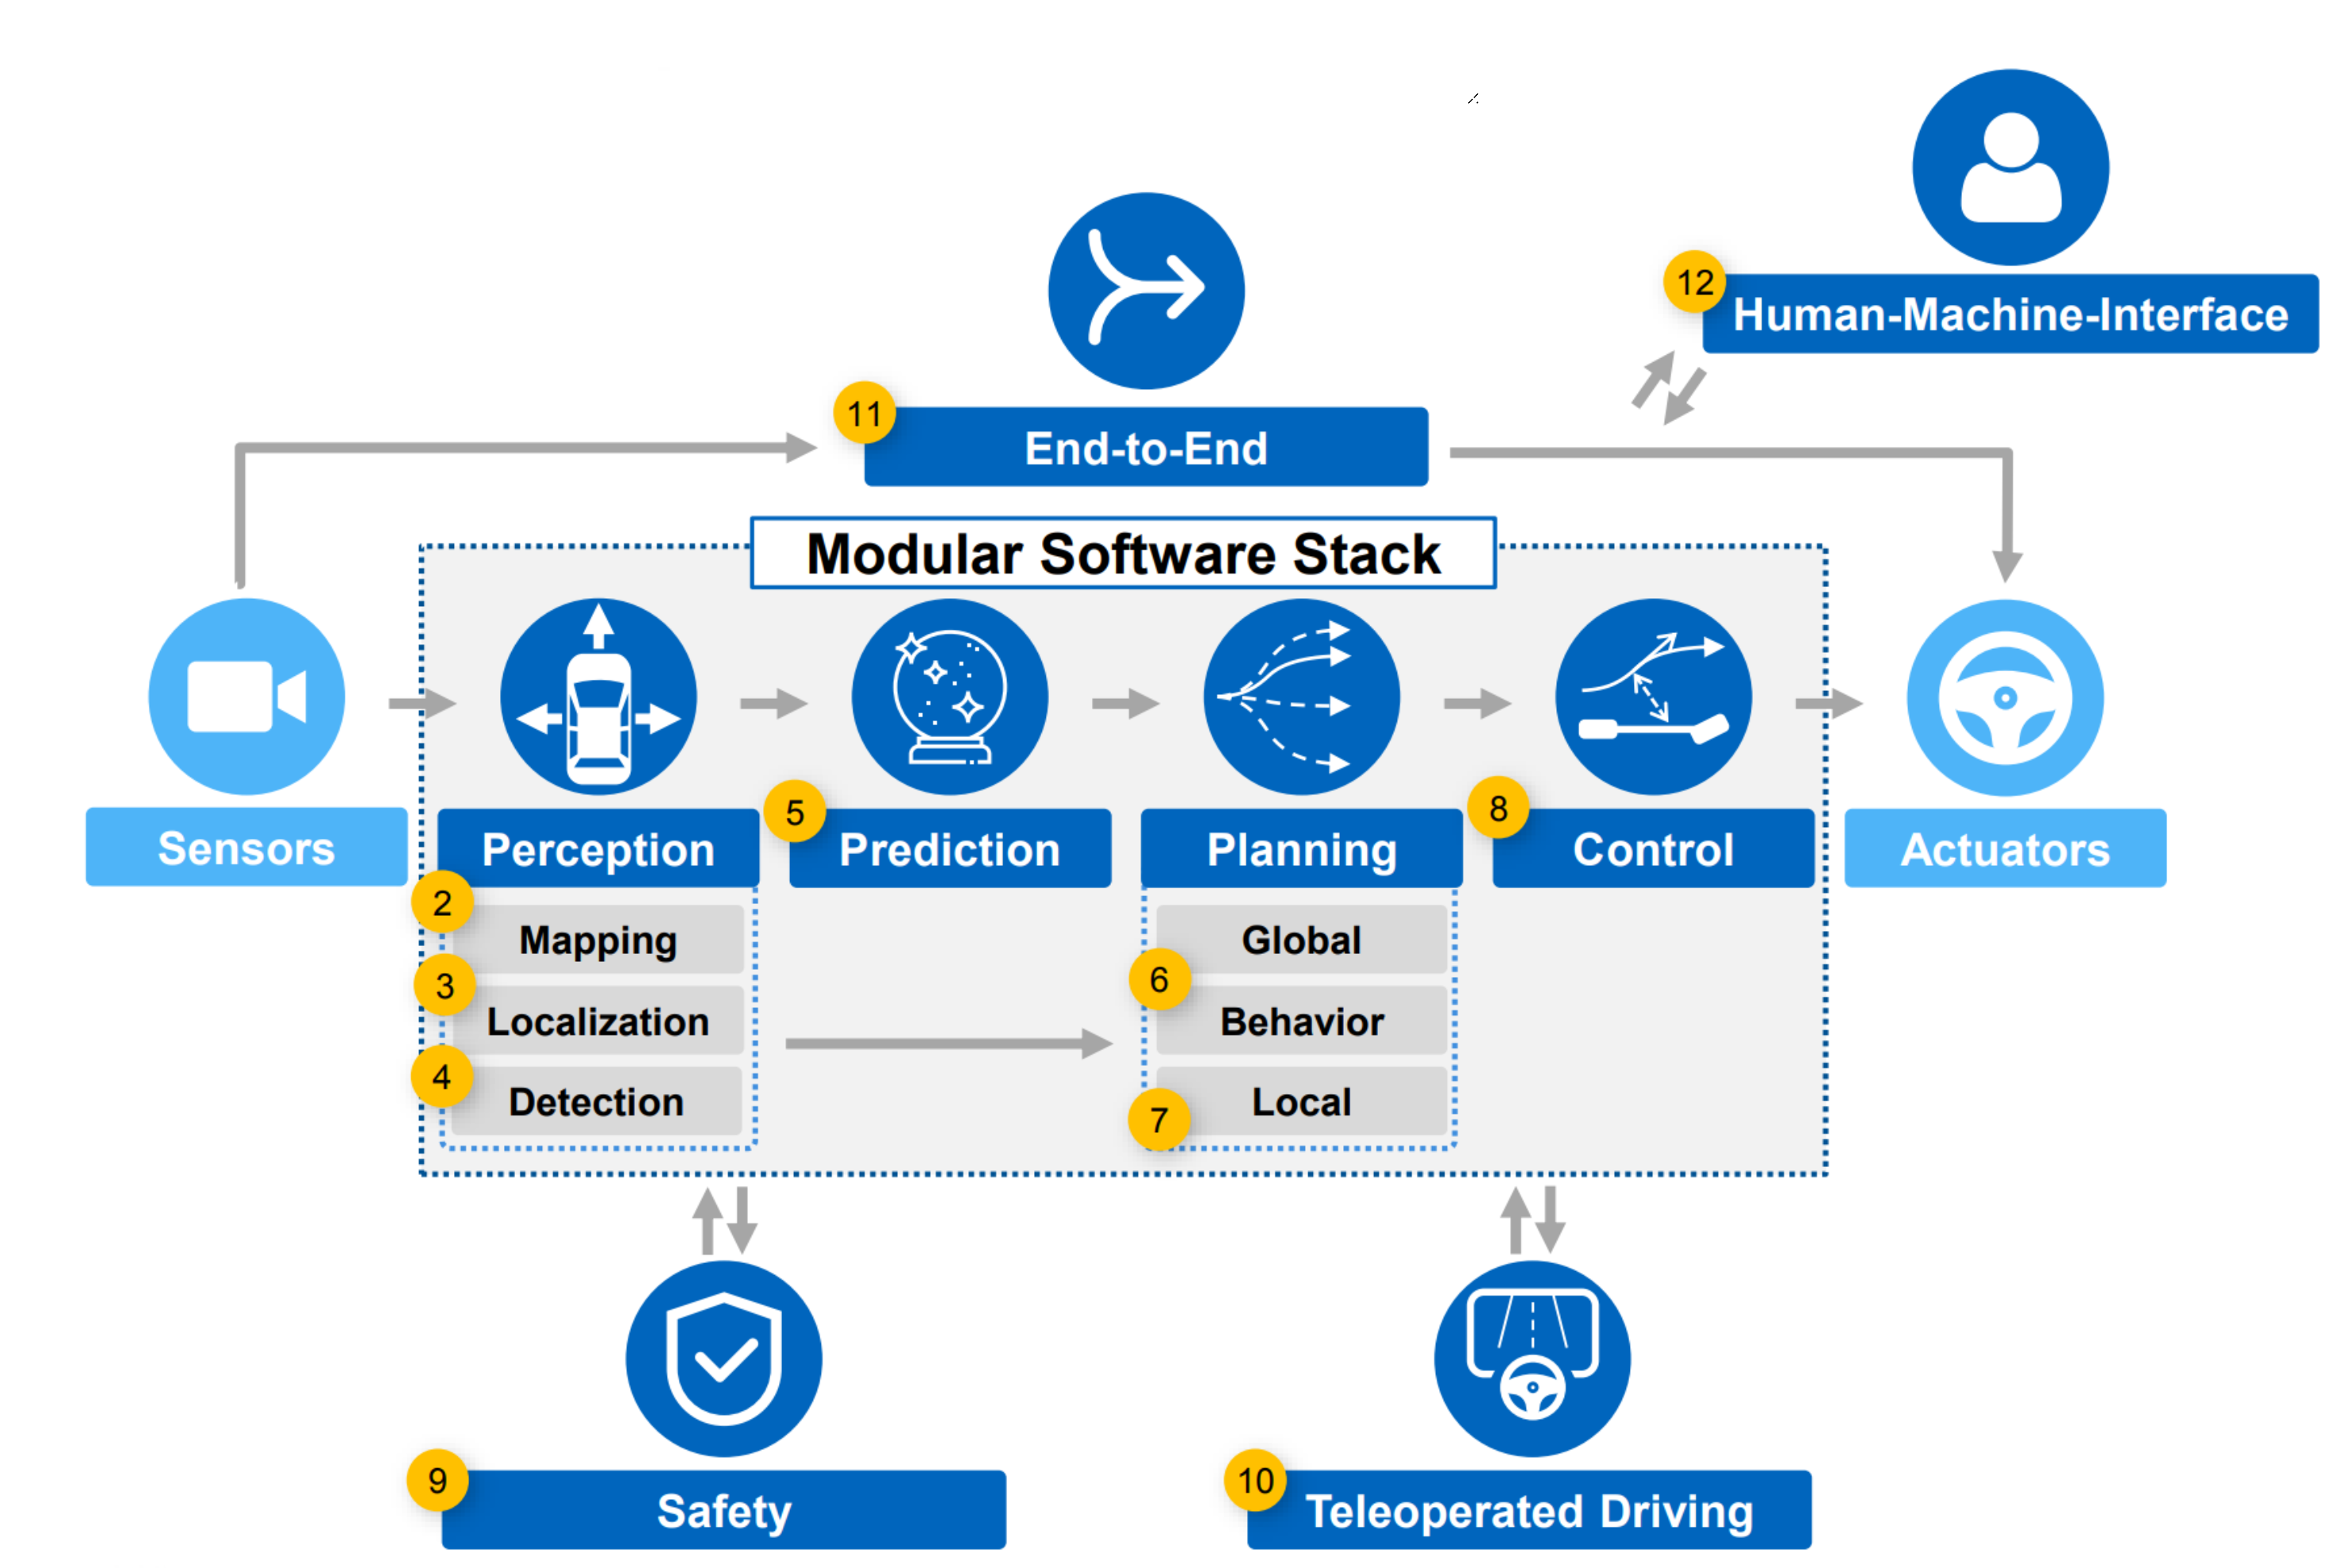
\includegraphics[scale=0.14]{figures/AVStack.png}
    \centering
    \caption{Autonomous Vehicle Technology Stack} %todo: add source from the lecture
    \label{fig:AVStack}
\end{figure}

While some research has explored end-to-end learning, where deep learning models directly map sensor inputs
to control outputs without modular decomposition \cite{codevilla2019limitations}, this approach alone is often
insufficient for achieving higher levels of autonomy. End-to-end systems can struggle with interpretability
and adaptability across diverse driving scenarios \cite{e2e}. It is an active research area and some
of the mentioned issues can be solved with Modular end-to-end learning \cite{nvidia2022diffstack} and also
it is expected to have a better performance on end-to-end methods with the improving hardware and datasets overtime \cite{e2e}.

For a system to reach higher SAE levels—particularly Level 4 or 5—all of
these modules must function reliably across various environments and conditions.
Each component plays a critical role in ensuring that the vehicle can navigate complex urban
environments safely and efficiently while responding to dynamic changes in real-time.
And we have teleoperation for the the cases where one or more module fails to deal the edge cases in the designed level of autonomy.
Teleoperation serves as a bridge between current autonomous driving capabilities and fully autonomous operation.
It allows vehicles to complete their missions even when their onboard systems encounter limitations.
For instance, if an autonomous vehicle encounters a situation outside its Operational Design Domain (ODD)\cite{iso34503},
such as unclear road markings or interactions with law enforcement, it can pull over safely and request human
intervention through teleoperation. This technology is essential for ensuring that autonomous vehicles
can operate reliably in real-world conditions and is expected to play a key role in the widespread adoption of autonomous vehicles.


\subsection{Types of Sensor Data in Autonomous Vehicles} \label{subsection:sensors}
Autonomous vehicles rely on a range of sensors to perceive their environment and
gather the necessary data for safe and efficient navigation. These sensors provide
raw data that is processed by the vehicle's perception system to understand its
surroundings, detect obstacles, and make real-time decisions.
In the later sections we will refer these unprocessed data as "Raw data" or "Raw sensory data".
The key types of sensor data used in autonomous vehicles include:
\begin{itemize}
    \item \textbf{LiDAR (Light Detection and Ranging):}
    LiDAR sensors use laser pulses to measure distances between the vehicle and surrounding objects.
    By emitting laser beams and measuring the time it takes for them to reflect back, LiDAR creates
    a detailed 3D map of the environment. This technology is particularly useful for detecting objects'
    shapes, sizes, and positions with high accuracy, even in low-light conditions \cite{levinson2011towards}.
    LiDAR is widely used in autonomous vehicle systems due to its precision in mapping the surrounding area.

    \item \textbf{Radar}:
    Radar sensors use radio waves to detect objects and measure their speed and distance from the vehicle.
    Unlike LiDAR, radar is less affected by adverse weather conditions such as rain or fog, making it a
    reliable sensor for detecting moving objects like other vehicles or pedestrians \cite{patole2017automotive}.
    Radar is often used for functions like adaptive cruise control and collision avoidance.
    \item \textbf{Cameras}:
    Cameras capture visual data from the environment, providing rich information about road signs,
    lane markings, traffic lights, and other vehicles. Autonomous vehicles typically use multiple cameras positioned
    around the vehicle to achieve a 360-degree view \cite{geiger2012we}. Cameras are crucial for tasks requiring
    high-resolution visual data, such as object classification and scene understanding.
    \item \textbf{Ultrasonic Sensors}:
    Ultrasonic sensors are commonly used for short-range detection tasks like parking assistance or detecting nearby
    obstacles at low speeds. These sensors emit sound waves and measure their reflections to detect objects within
    a few meters of the vehicle \cite{zhang2018ultrasonic}.
    \item \textbf{GPS (Global Positioning System)}:
    GPS provides location data by triangulating signals from satellites. While GPS alone may not offer the precision
    required for autonomous driving, it is often combined with other localization methods such as SLAM
    (Simultaneous Localization and Mapping) to improve accuracy \cite{thrun2005slam}.
    \item \textbf{IMU (Inertial Measurement Unit)}:
    The IMU measures the vehicle's acceleration and angular velocity using accelerometers and gyroscopes.
    This data helps track the vehicle's movement and orientation in real time, contributing to accurate
    localization when combined with GPS data \cite{madgwick2011imu}.
\end{itemize}

We referenced a subset of TUM's EDGAR research vehicle's sensor setup as our basis.
EDGAR is equipped with 10 camera sensors, 4 LIDAR sensors (long and short-range), 6 RADAR sensors as well as GPS, IMU (Inertial Measurement Unit) and microphones \cite{tum2023edgar}

\subsection{Perception Systems in Autonomous Vehicles}
Perception systems are an essential component of autonomous vehicles, responsible for interpreting the
vehicle's surroundings and enabling safe navigation. These systems process data from sensors such as LiDAR,
radar, and cameras to detect and classify objects, track their movements, and localize the vehicle within
its environment \cite{liu2018perception}. The perception system builds a comprehensive model of the environment,
which is then used by other modules—such as prediction, planning, and control—to make driving decisions.

This thesis will refer to "Perception Data" as the processed output from the vehicle's perception system. This includes information about detected objects (e.g., vehicles, pedestrians), their classifications, positions, and trajectories. The perception system also generates high-level semantic information such as lane markings, traffic signs, and road boundaries. This data enables autonomous vehicles to understand their environment and make informed decisions.

We utilize Autoware, an open-source software stack designed for autonomous driving systems for all perception-related tasks in this project. Autoware provides a comprehensive set of tools for processing sensor data and generating perception outputs \cite{kato2018autoware}. It includes object detection, classification, tracking, and localization modules using sensors such as LiDAR, radar, and cameras. By leveraging Autoware's robust perception capabilities, we ensure that our system can handle complex environments while maintaining flexibility for future improvements.

Autoware also supports sensor fusion techniques that combine data from multiple sensors to improve accuracy and reliability. This is especially important when dealing with noisy or incomplete sensor data. For instance, Autoware's fusion algorithms can combine LiDAR point clouds with radar measurements to enhance object detection
performance in adverse weather conditions where cameras may struggle.
\section{Teleoperation Concepts}

Teleoperation is an essential fallback solution for autonomous vehicles (AVs),
enabling a human operator to remotely assist or take control of a vehicle when
its automated systems encounter situations beyond their operational design domain (ODD)
or face disengagements. These scenarios often arise due to complex or unforeseen edge cases,
such as sensor malfunctions, unanticipated obstacles, or ambiguous road conditions.
ensuring that it can resume its mission safely and efficiently \cite{Brecht}.

Several teleoperation concepts have been developed to address different aspects of remote vehicle control, each with its own strengths and limitations. These concepts can be broadly categorized into Remote Driving, Remote Assistance, and Perception Modification. Each approach targets specific challenges in teleoperation, such as latency, situational awareness, and operator workload.

\subsection{Remote Driving}
Remote Driving is one of the earliest teleoperation concepts,
where a human operator takes full control of the vehicle's
dynamic driving tasks (DDT), including steering, acceleration,
and braking. This concept has been explored for more than two decades.
Early research by Sworder et al. \cite{sworder1999performance} (1999) demonstrated the feasibility
of teleoperating vehicles using direct control methods, where
operators manually control vehicles based on live video feeds and
sensor data transmitted from the vehicle to a remote station.
This method, known as Direct Control, has been widely studied
and implemented in various industries since then.

Despite its long history, Direct Control remains relevant
today due to its simplicity and directness. In this approach,
the operator receives real-time video and sensor data from the
vehicle and sends back control commands such as steering angles
or velocity adjustments. However, this method is highly sensitive
to network conditions—particularly latency and bandwidth
limitations—which can lead to reduced situational awareness for
the operator and delayed reactions to dynamic situations \cite{Gnatzig}.
Latency is a critical factor in teleoperation; studies have shown
that latencies greater than 100 milliseconds can result in degraded
performance in high-speed or complex environments \cite{chucholowski2014teleoperated}.
Under fluctuating network conditions—such as handovers
between cellular towers or signal degradation due to obstacles—latency
can increase unpredictably, leading to delayed responses that
compromise safety \cite{neumeier2023feasibility}.

In recent years, several companies have implemented Direct Control
in real-world applications despite these challenges. For example,
Fernride, a Munich-based company, has successfully deployed
teleoperation technology for logistics operations. Fernride's
platform allows remote operators to control semi-autonomous
trucks in logistics yards using Direct Control methods.
In their pilot project with DB Schenker and KAMAG,
teleoperators remotely controlled trucks for yard shunting
tasks—moving trailers around loading docks—demonstrating that
teleoperation can be safely integrated into existing logistics
processes \cite{fernride2023}. The success of this project
highlights the potential of Direct Control in controlled
environments like logistics yards where network conditions are stable.

However, while Direct Control has proven effective in specific use cases
such as logistics yards or industrial environments with
controlled network conditions, it faces significant challenges when
applied to more complex or dynamic environments like urban roads.
The sensitivity of Direct Control to network latency makes it less
suitable for scenarios where real-time decision-making is critical for
safety. To mitigate these challenges, modern teleoperation systems
often incorporate additional safety measures or alternative methods
that reduce reliance on real-time control inputs.

One such alternative is Shared Control, where the vehicle retains
some level of autonomy while the operator provides high-level
inputs. In this approach, if an operator's input does not meet
certain safety criteria—such as proximity to other vehicles—the
vehicle's onboard systems can override those commands to prevent
collisions \cite{kay2024sharedcontrol}. This approach reduces
cognitive load on the operator while ensuring that safety-critical
decisions are still handled by the vehicle's autonomous systems.

\subsection{Remote Assistance}
Remote Assistance focuses on providing high-level guidance or support
to specific functions of the AV without taking full control of the DDT.
This method is often used in scenarios where the AV encounters an
edge case that prevents it from continuing its mission autonomously
but does not require complete human intervention.

In Waypoint Guidance, for example, operators provide waypoints or general
directions for the vehicle to follow while leaving detailed path planning
and execution to the AV's onboard systems \cite{corridor}. This reduces
operator workload but may lead to stop-and-go behavior if communication
between the operator and vehicle is not seamless.

Another promising approach is Collaborative Planning, where operators
work with the AV's planning system by selecting from a set of pre-generated
path suggestions based on sensor data. This method allows operators to focus
on decision-making rather than low-level control tasks \cite{hosseini2024collaborative}.
Collaborative planning improves efficiency but requires robust sensor fusion and reliable
perception data from the AV.
\subsection{Perception Modification}

Perception Modification is one of the most promising teleoperation
concepts, designed to address situations where an autonomous
vehicle (AV) encounters perception errors that prevent it
from continuing its mission. These errors may arise from false
positives or misclassifications in the vehicle's perception system,
such as detecting an object that is not truly obstructing the path or
misinterpreting environmental features like lane markings or road signs.
In such cases, Perception Modification allows a remote operator to
intervene by modifying how the AV interprets its environment,
enabling it to resume its journey \cite{feiler2023perception}.

In this concept, the operator has access to both raw sensor data
(e.g., LiDAR point clouds or camera images) and processed perception
data (e.g., object classifications or environmental models).
By reviewing this data, operators can identify discrepancies
between what the vehicle perceives and what is present in its
surroundings. For example, if a false-positive detection is blocking
the vehicle's path—such as a plastic bag being detected as a solid
obstacle—the operator can modify or correct these perceptions by
marking the area as drivable. This correction enables the AV to
continue its mission without requiring complete manual control \cite{feiler2023perception}.

The Perception Modification concept is beneficial because
it reduces the cognitive load on the operator compared to direct control methods.
Instead of managing all aspects of driving, operators focus solely on correcting
specific perception errors. This approach allows for more efficient human
intervention while minimizing the risk of operator fatigue or error due to
high mental workload \cite{Brecht}. Additionally, Perception Modification can
be extended beyond object detection corrections; operators could also modify other
aspects of the environmental model, such as lane boundaries or drivable space predictions.

As Feiler, et al. \cite{feiler2023perception} define it, the implementation of
Perception Modification involves integrating a  Human-Machine Interface (HMI) that provides operators with real-time access to both raw sensor data and processed perception data. The HMI allows operators to
mark areas as drivable or ignore specific detections deemed irrelevant or incorrect. The vehicle's planning module receives this modified perception data and generates a new trajectory based on these corrections.

In their comparative study of teleoperation concepts, Brecht et al. \cite{Brecht} found
that Perception Modification imposes less cognitive load on operators than
Direct Control while still enabling efficient resolution of disengagements.
The study also highlighted that Perception Modification is highly effective in
situations where false-positive detections or indeterminate objects hinder an AV's progress.
However, it may not be suitable for all disengagement scenarios—particularly those
involving complex trajectory planning failures or situations requiring immediate manual intervention.

\section{Environmental Data Visualization for Autonomous Vehicles}
Environmental data visualization plays a fundamental role in autonomous vehicle systems,
particularly in teleoperation scenarios where human operators must understand and interpret
complex sensor data to make critical decisions. Visualizing environmental data is crucial
for two reasons: First, it enables operators to maintain high situational awareness during
teleoperation tasks \cite{Gnatzig}. Second, it allows for effective monitoring and verification
of the vehicle's perception system, essential for identifying and correcting potential errors
in the automated driving system \cite{feiler2023perception}.

\subsection{Challenges in Visualizing Multi-Sensor Data}
One of the primary challenges in environmental data visualization is integrating data from multiple
sensors into a cohesive representation of the environment. Modern autonomous vehicles generate
massive amounts of data - up to 3-6 TB of raw data per hour of operation from their sensor suite \cite{kazhamiaka2021challenges}
. A single 4K camera operating at 30 frames per second can produce
approximately 5.4 TB per hour, while a typical AV may have 6-12 cameras along with other sensors \cite{visualcapitalist2024}
. This creates a significant challenge in data processing, transmission,
and visualization. Each sensor type has strengths and limitations, as we defined in section \ref{subsection:sensors}.

The sensor fusion process combines these different data streams into a single, a unified environmental
model that is used by nearly all parts of the autonomous driving stack like perception system \cite{feng2020deep}
, localization system \cite{feng2020deep, el-sheimy2020sensorfusion}. It can also be used for the human operator interface.
However, visualizing this fused data presents several challenges:
\begin{itemize}
    \item \textbf{Data Overload:} Presenting all sensor data simultaneously can overwhelm operators with too much information. With autonomous vehicles generating up to 10 exabytes of monthly data across a fleet, effective visualization techniques must prioritize relevant information while filtering out unnecessary details \cite{visualcapitalist2024}. % todo: revisit
    \item \textbf{Real-Time Processing:} Processing and visualizing sensor data in real time requires significant computational resources. Delays in processing can lead to outdated information being presented to the operator, reducing situational awareness \cite{Gnatzig}.
    \item \textbf{Accuracy vs. Latency:} High-fidelity visualizations may improve accuracy but come at the cost of increased latency. A balance between these two factors must be kept for effective teleoperation \cite{chucholowski2014teleoperated}.
\end{itemize}

Data overload is particularly sensitive in teleoperation scenarios, where operators must quickly understand and respond to complex environmental data while maintaining real-time awareness of the vehicle's situation. This requires careful consideration of which data to present and how to present it effectively without overwhelming the operator's cognitive capabilities.

\subsection{Human Factors in Perception Data Visualization}

\section{Existing Approaches to Visualizing Sensor Data}
\subsection{Industry Standards}
\subsection{TOD Visual 2.0}
\subsection{Separate View}\label{section:separateview}
\subsection{Integrated View Approaches}\label{section:integratedview}
\subsection{NeRF-based rendering methods}
\subsection{Depth Completion}

\section{User Experience and Interface Design for Autonomous Vehicles}
\subsection{Human-Machine Interaction in Autonomous Vehicles}
\subsection{User-Centered Design Principles for Vehicle Interfaces}
\subsection{Cognitive Load and Information Processing in Driving Scenarios}
\subsection{Situational Awareness in Teleoperation}

\section{Evaluation Methods for Visualization Concepts}
\subsection{Usability Testing Techniques}
\subsection{Performance Metrics for Visualization Effectiveness}
\subsection{User Studies in Automotive Interface Design}

\section{Summary}
\subsection{Requirements}
\subsection{Research Gap}


